\documentclass[compress]{beamer}\usepackage{graphicx, color}
\usepackage{alltt}
\usepackage{wrapfig}	%in-line figures
\usepackage[square, comma, sort&compress]{natbib}		%bibliography
\usepackage{pslatex} 	%for times new roman
\usepackage[parfill]{parskip}    % Activate to begin paragraphs with an empty line rather than an indent
\usepackage{graphicx}
\usepackage{amssymb}
\usepackage{epstopdf}
\usepackage{booktabs}
\usepackage{amsmath}
\usepackage{color} % for coloring of text
\usepackage{multirow}
\usepackage{outlines}
\usepackage{xfrac}
\usepackage{relsize} % for scaling parts of equations. e.g. \mathlarger
\usepackage{hyperref}
\usepackage{rotating}
\usepackage{array} 
\usepackage{moresize}

\DeclareGraphicsRule{.tif}{png}{.png}{`convert #1 `dirname #1`/`basename #1 .tif`.png}
\usetheme{Singapore}
\setbeamertemplate{caption}[numbered]

\providecommand{\e}[1]{\ensuremath{\times 10^{#1}}}

\begin{document}

\newcommand{\multilineR}[1]{\begin{tabular}[b]{@{}r@{}}#1\end{tabular}}
\newcommand{\multilineL}[1]{\begin{tabular}[b]{@{}l@{}}#1\end{tabular}}
\newcommand{\multilineC}[1]{\begin{tabular}[b]{@{}c@{}}#1\end{tabular}}

\section{Introduction}
\subsection{Title}
\begin{frame}

%Interpreting metabolism at the interface of the metabolome and proteome: A metabolism-wide approach to identifying physiologically-relevant metabolic regulation and understanding flux control
%An integrated �omics approach to large-scale quantitative analysis of cellular metabolic regulation
\frametitle{\footnotesize{How metabolite and enzyme concentrations jointly drive flux: Integration of steady-state metabolite, enzyme and flux measurements points to the nature of flux control and enables the identification of physiologically-relevant metabolic regulation}}

\footnotesize{Abstract}

\ssmall{
Rates of metabolic reactions are driven by changes in enzyme activity and metabolite abundance, a simply relationship, which belies the complexity that arises when thousands of such metabolites and enzymes interact, collectively constructing a cell's metabolism.  To simplify this complexity, we were able to break the dependence between metabolite and enzymes abundances and metabolic rates (fluxes) through experimental measurement of these concentrations and fluxes.  In such a situation, if we knew the true \textit{in vivo} kinetic form of reactions, then we could use this form to map measured abundances of reaction species to metabolic rates.  Instead, we solved the inverse problem: inferring the form of metabolic reactions having measured reaction species and rates across a set of 25 steady-state conditions.  For 17 reactions, flux predicted from Michaelis-Menten kinetics, informed by concentrations of substrates, products, enzymes, was consistent with measured flux.  For 28 additional reactions, a consistent relationship was possible once regulation by small molecules was added.  These regulatory interactions largely reproduce regulation that is well supported in the literature such as feedback control of amino acid biosynthesis, but for five reactions further investigation was warranted.  We find that there is a physiological role of aliphatic amino acids inhibiting Ornithine Transcarbamylase. Using approximately correct reaction forms for 45 reactions we were able to explain how variable flux through each reaction is driven by changes in substrates, products, enzymes and regulators and find that changes in flux are primarily caused by changes in metabolite concentrations.  This suggests that metabolism is a self-regulating system, controlled by the nutrient environment and fine-tuned by the transcriptional network.}

\end{frame}

\subsection{Overview}

\begin{frame}

\frametitle{Outline of Figures}
\begin{outline}
\1 F1: Proteome-wide variation.
\1 F2: Metabolism-wide flux prediction.
\1 F3: Alignment of measured flux, metabolite concentrations and enzymes using just simple Michaelis-Menten kinetics.
\1 F4: Other reactions require the addition of small molecule regulators to show consistency.
\1 F5: Summary of performance at the level of 55 reactions.
\1 F6: Using this method to identify novel regulation.
\1 F7: Control of flux
\end{outline}

\end{frame}

% Annotate irreversibility in comparison to allostery
% Label individual reactions that are allosteric
% Check Aconitase and other reactions which are less sure
% Clearer labelling of ternary plot
% ASL ihibition by arginine
% UTP GUT substrate inhibition

% Pay someone to synthesize Ura3
% ARG3 - need to leave out Leucine and see how it looks
% Negative feedback transfer metabolic control from the supply to the demand

% Bringing biochemistry into physiology - which experimentally determined regulators are artifacts and which are actually regulating flux
% How to determine what this one thing is - highly dependent on concentrations tests and difficult experiments are required
% Metabolism is simple - changes in substrates and products and maybe one other thing - which may be greatly important

\section{Figures}

\subsection{F1}
\begin{frame}
\vspace{2mm}
\begin{figure}[h!]
      \begin{columns}
        \column{.3\linewidth}
        \caption{Relative abundance (log$_{2}$) of 1187 proteins across 25 nutrient conditions.  Each row was mean-centered and hierarchically-clustered based on pearson correlation}
        \column{.55\linewidth}
        \includegraphics[width=\textwidth]{Figures/F1-proteinHM.pdf}
        \label{fig:proteinHM}
      \end{columns}
\end{figure}
\end{frame}

\subsection{F2}
\begin{frame}
\vspace{2mm}
\begin{figure}[h!]
      \begin{columns}
        \column{.3\linewidth}
        \caption{Flux through 233 reactions across 25 nutrient condition relative to the median flux for each reaction.  Reactions were hierarchically-clustered using spearman correlation}
        \column{.55\linewidth}
        \includegraphics[width = 0.85\textwidth]{Figures/F2-fluxHM.pdf}
        \label{fig:fluxHM}
      \end{columns}
\end{figure}
\end{frame}

\subsection{F3}
\begin{frame}
\vspace{2mm}
\begin{figure}[h!]
      \begin{columns}
        \column{.3\linewidth}
        \caption{Flux through triosephosphate isomerase can be explained using Michaelis-Menten kinetics.}
        \column{.55\linewidth}
        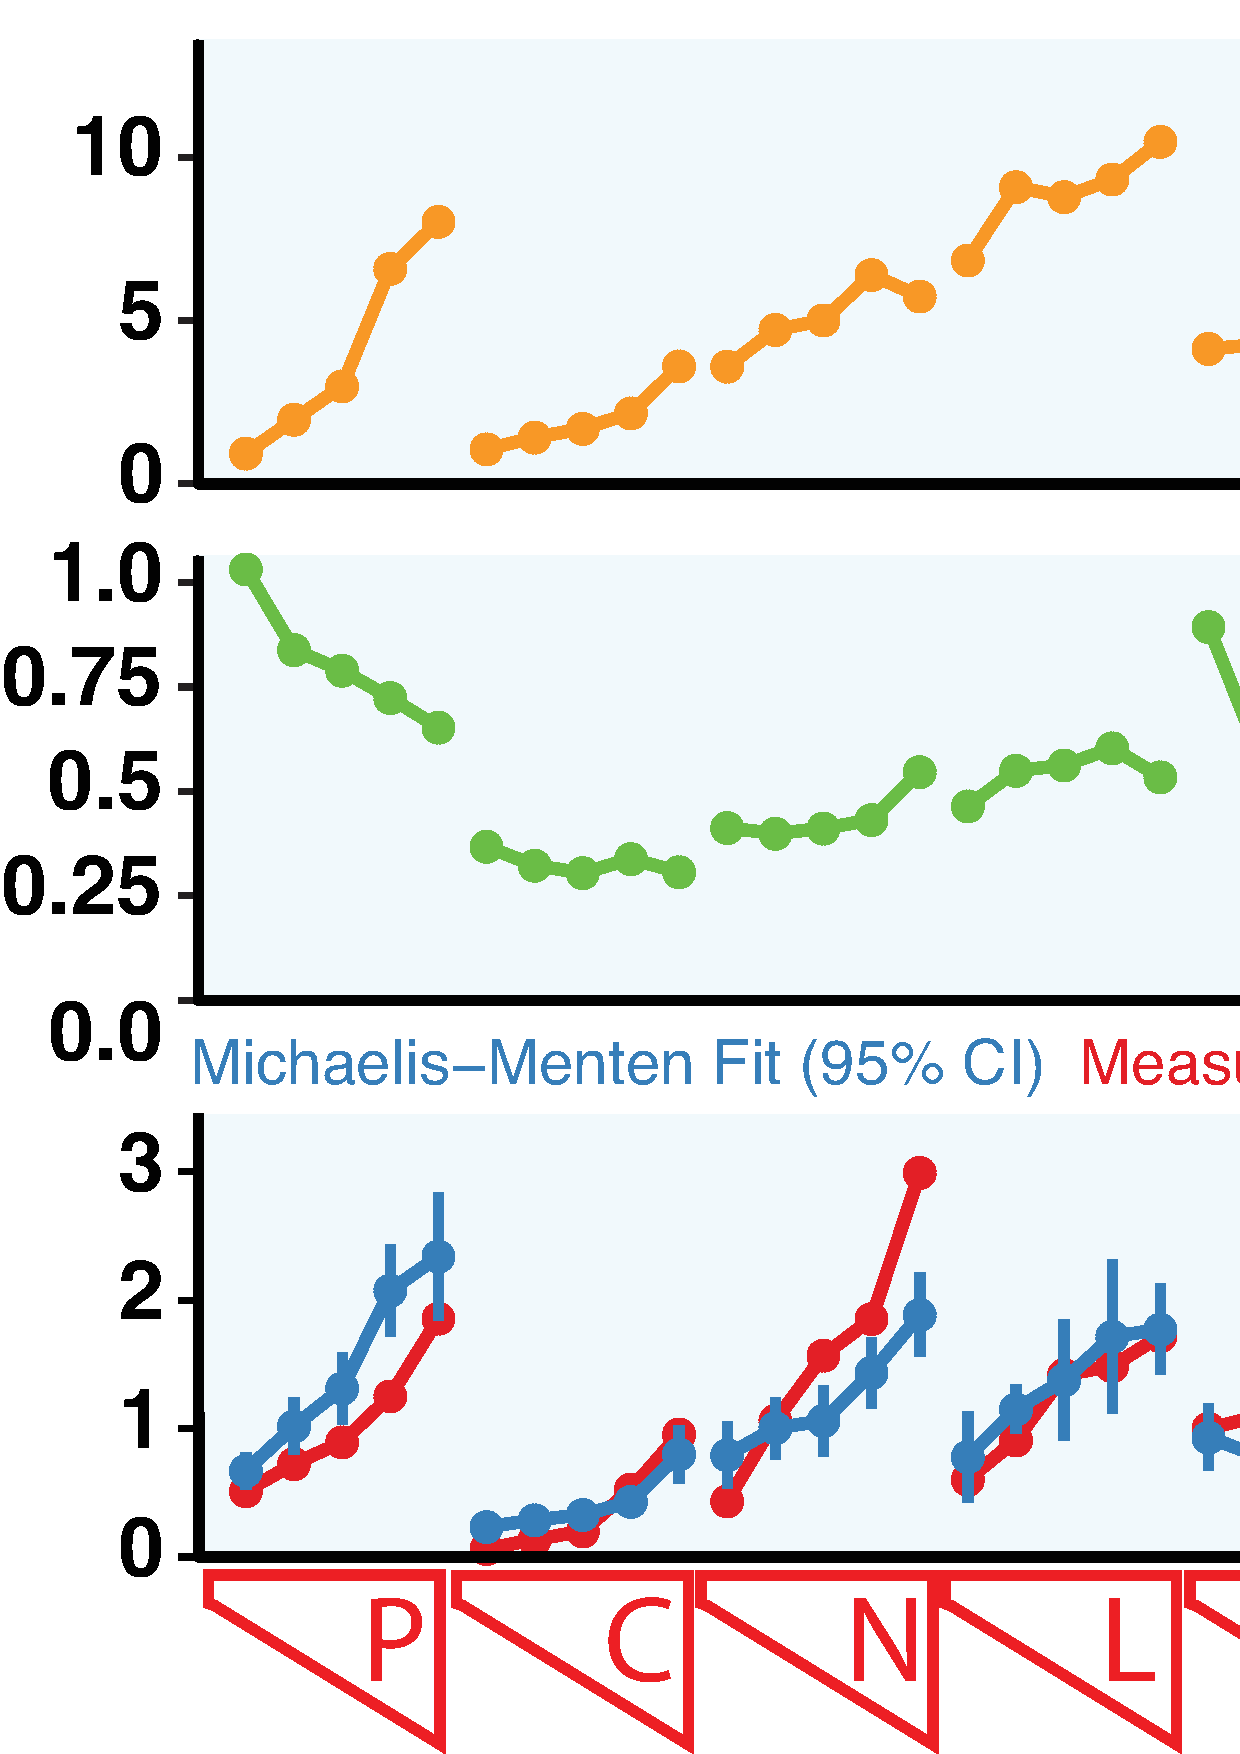
\includegraphics[width = 0.9\textwidth]{Figures/F3-MMkinetics.pdf}
        \label{fig:TPI}
      \end{columns}
\end{figure}
\end{frame}

\subsection{F4}
\begin{frame}
\vspace{2mm}
\begin{figure}[h!]
      \begin{columns}
        \column{.3\linewidth}
        \caption{Pyruvate kinase flux is not consistent with a Michaelis-Menten function of the substrates, products and isoenzymes.  The addition of fructose-1,6-bisphosphate as an allosteric activator results in a close consistency between predicted and measured flux.}
        \column{.65\linewidth}
        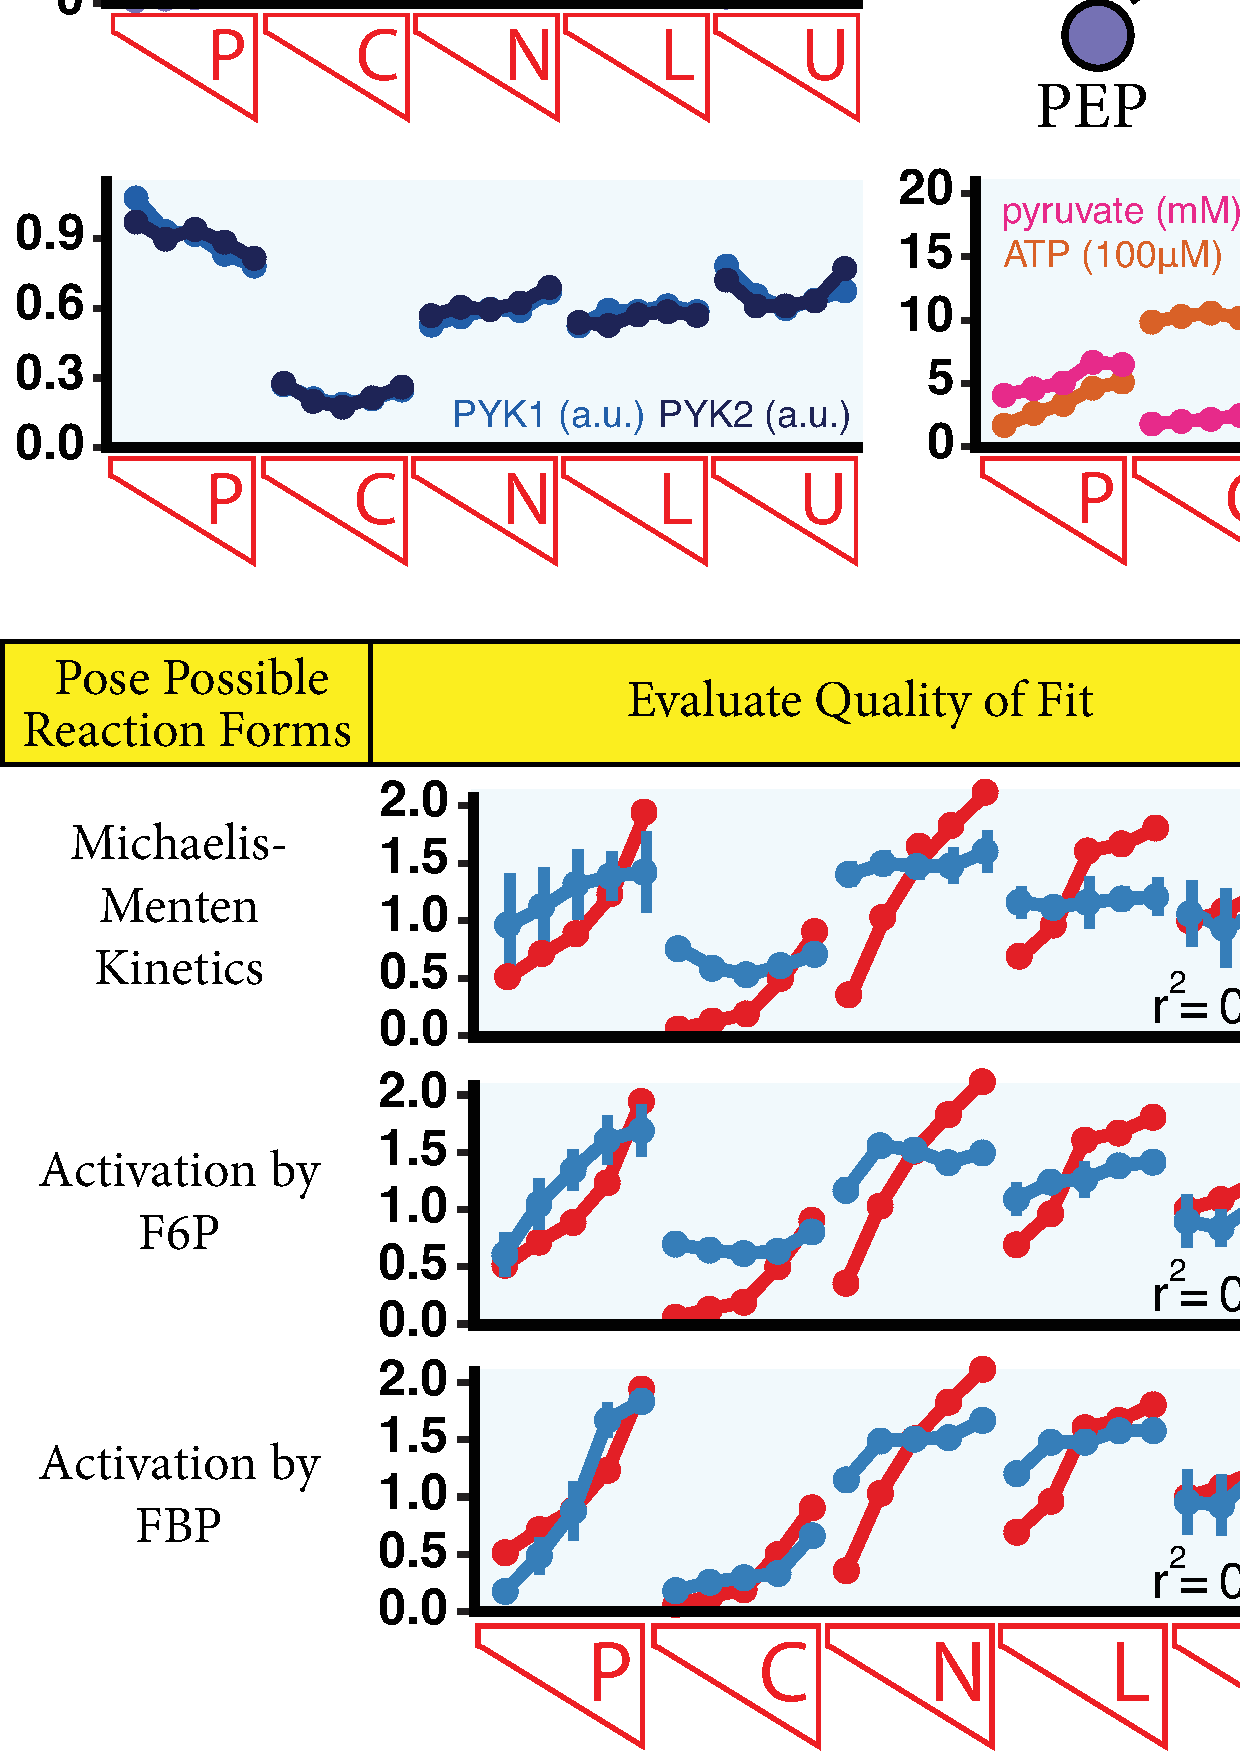
\includegraphics[width = \textwidth]{Figures/F4-identifyingRegulation.pdf}
        \label{fig:PYK}
      \end{columns}
\end{figure}
\end{frame}

\subsection{F5}
\begin{frame}
\vspace{2mm}
\begin{figure}[h!]
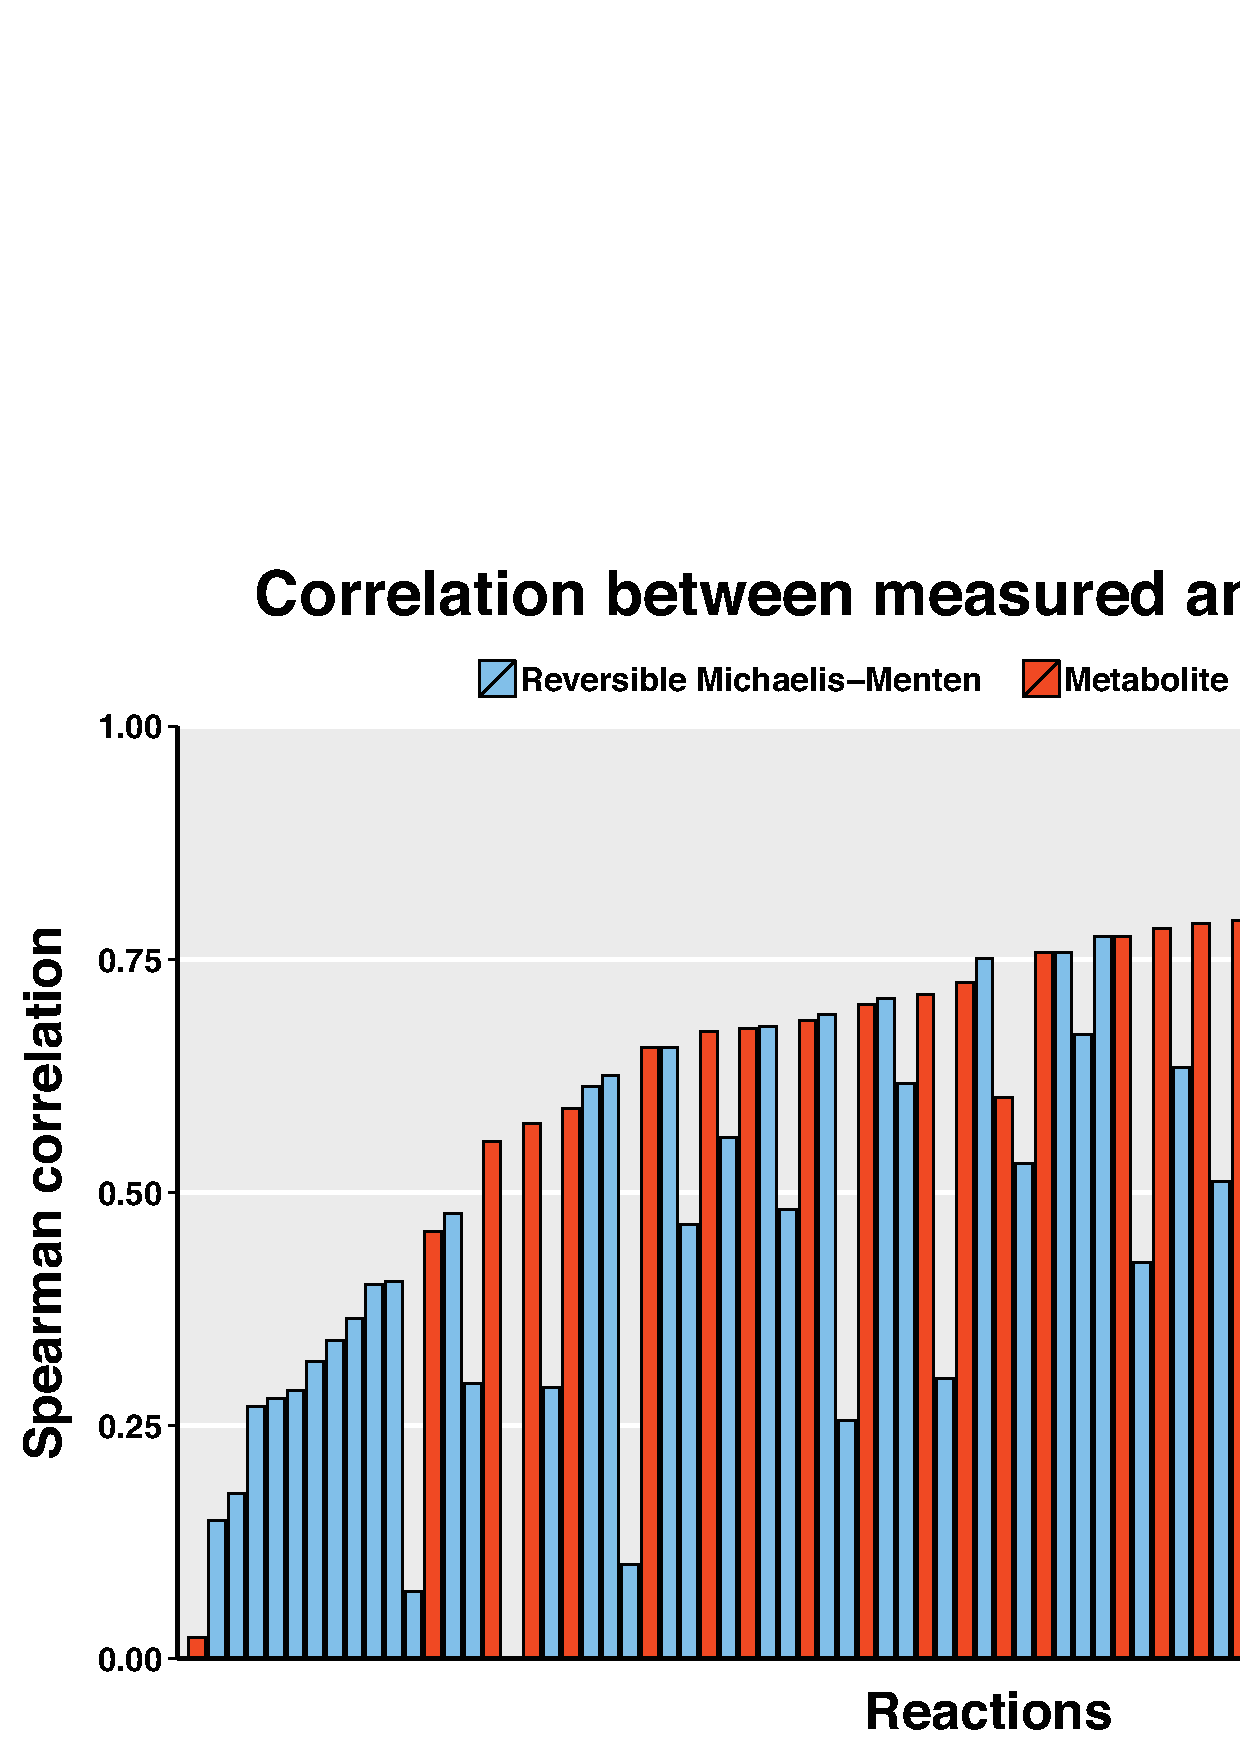
\includegraphics[width = 0.8\textwidth]{Figures/F5-reactionFits.pdf}
\caption{Metabolism-wide summary of the consistency between measured flux and Michaelis-Menten predictions.  Each of 55 reactions is compared using just simple Michaelis-Menten kinetics as well as by adding the most statistically significant regulator (if one exists)}
\label{fig:reactionFits}
\end{figure}
\end{frame}

\subsection{F6}
\begin{frame}
\vspace{2mm}
\begin{figure}[h!]
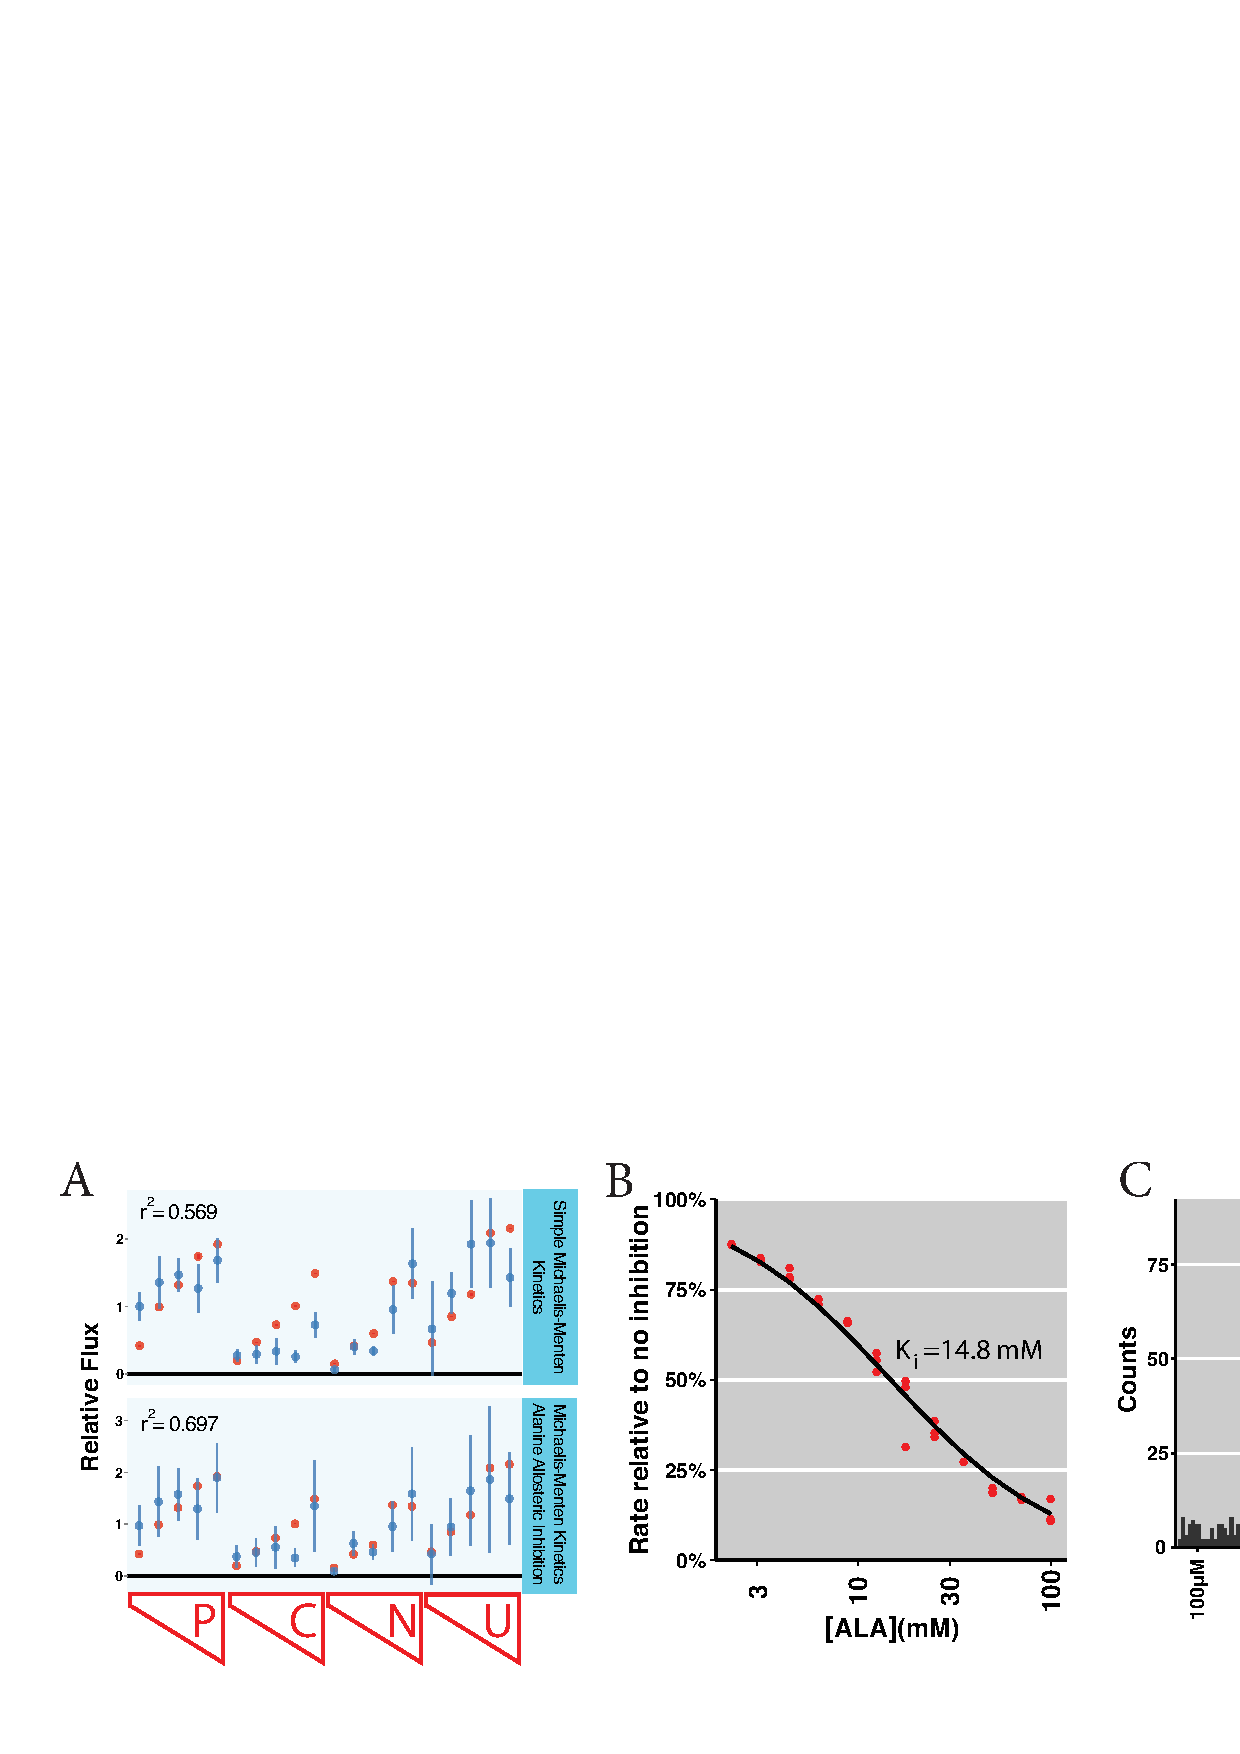
\includegraphics[width = 1\textwidth]{Figures/F6-OTCaseKinetics.pdf}
\caption{Alanine is a physiological regulator of ornithine carbamoyltransferase.  \textbf{A)} The kinetic prediction with the addition of Alanine results in a statistically-significant improvement in fit relative to simple Michaelis-Menten kinetics. \textbf{B)} \textit{In vitro} measurement of the impact of alanine concentration on OTCase indicates that alanine is an allosteric inhibitor with a k$_{i}$ of 14.8mM.  \textbf{C)} Experimental and inferred k$_{i}$ values strongly agree and indicate that at measured concentrations. Alanine has an appropriate affinity and concentration to act as a physiological inhibitor of OTCase.}
\label{fig:OTCaseKinetics}
\end{figure}
\end{frame}

\subsection{F7}
\begin{frame}
\vspace{2mm}
\begin{figure}[h!]
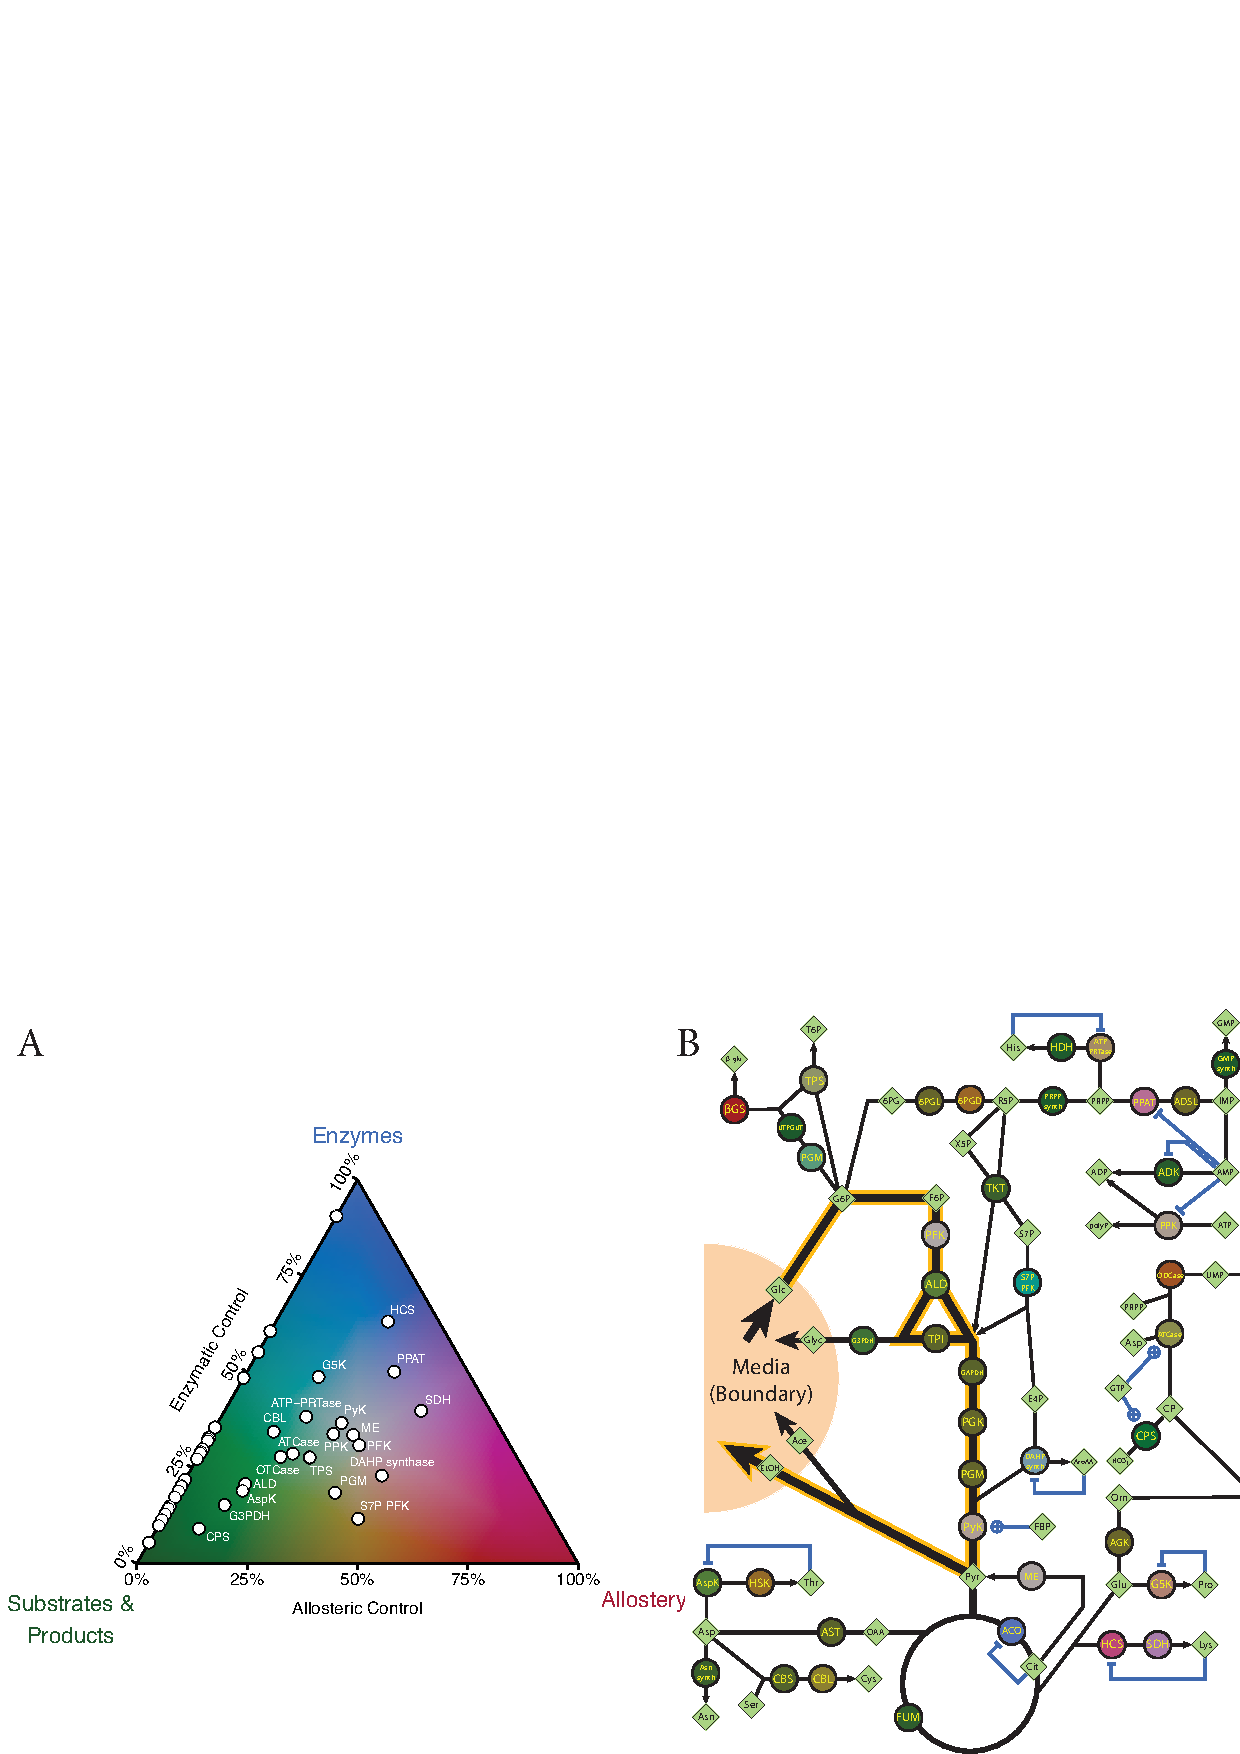
\includegraphics[width = 1\textwidth]{Figures/F7-metabolicLeverage.pdf}
\caption{\scriptsize{Each reaction was summarized based on the relative extent to which substrates/products, enzymes and allostery drive flux.  \textbf{A)} Each reaction is placed on a ternary surface where reactions in the lower left are driven by variable concentrations of substrates and products, those in the top by changes in enzymes and those in the bottom right by changes in allosteric regulators.  \textbf{B)} The color assigned to each reaction in the ternary surface is used to color a metabolic diagram.}
\label{fig:metabolicLeverage}}
\end{figure}
\end{frame}

\end{document} 
